
\section[Statistics]{Statistical Interpretation of the results}\label{sect:stat}

Since no excess of data over the background prediction has been observed, 
we close our study with setting upper limits on the testing signals.
This is conducted using a modified frequentist approach, namely CLs method \cite{read:CLs}.
In this method, the test statistic $q_\mu$ \cite{cowan:asymptoticCLs} is a function of the profile likelihood-ratio,

\begin{align}
q_\mu = -2 \ln \frac{\mathcal{L}(data ;\, b + \mu s)}{\mathcal{L}(data ;\, b + \hat{\mu} s)},
\end{align}

where $\hat\mu$ is the \textit{signal strength modifier} $\mu$ at the maximum point of the likelihood $\mathcal{L}$.
Then CLs is given by the following probability-ratio,

\begin{align}
CL_s = \frac{p(q_\mu \geq q_\mu^{obs} | b + \mu s )}{p(q_\mu \geq q_\mu^{obs} | b)}.
\end{align}
 
We compute CLs using a software package provided by the CMS Higgs PAG \cite{higgspag:software}.
After incorporating systematic uncertainties, an observed CLs smaller than 0.05 for a signal strength of $\mu = 1$, excludes the given signal at $95\%$ CL. Indeed, the package determines which signal strength $\mu$ excludes the testing signal at $95\%$ CL. Therefore all resulting $\mu \leq 1$ define the excluded region in the parameter space of the given signal. 

In this analysis, we examine the data in three different channels.
These channels include tau-tau, muon-tau and electron-tau.
The signal region for the muon-tau and electron-tau channels is defined in one bin, which is $MT2 > 90$ and $tauMT > 200$ .
Due to the sensitivity of tau-tau channel to the signal, we look at the data in two different bins.
The first bin is $MT2 > 90$ and the second one is $40 < MT2 < 90$ and $sumMT>250$.
We eventually combine all four bins to to utilize more information from the observed and the predicted distributions.
Figures \ref{fig:limit_bins} show the impact of each bin on the combined result, represented by the final exclusion limit shown in Figure \ref{fig:limit_final}.  

To investigate the exclusion power of our research, we study the topology of direct stau pair production and  the $\PSGcpDo\PSGcmDo$ production in Simplified Models \cite{alves:sms}. 
Calculation of the expected exclusion limit shows that  
the research has potential to exclude 
%excludes 
a sizable region of the phase space, surrounded by the lines of $m_{\tilde{\chi}} = 500\GeV$ and $m_{\PSGczDo} = 150\GeV$ with an integrated luminosity of $19.6\,\fbinv$.


%%%%%%%%%%
\begin{linenomath}
\begin{figure}[h]
\centering
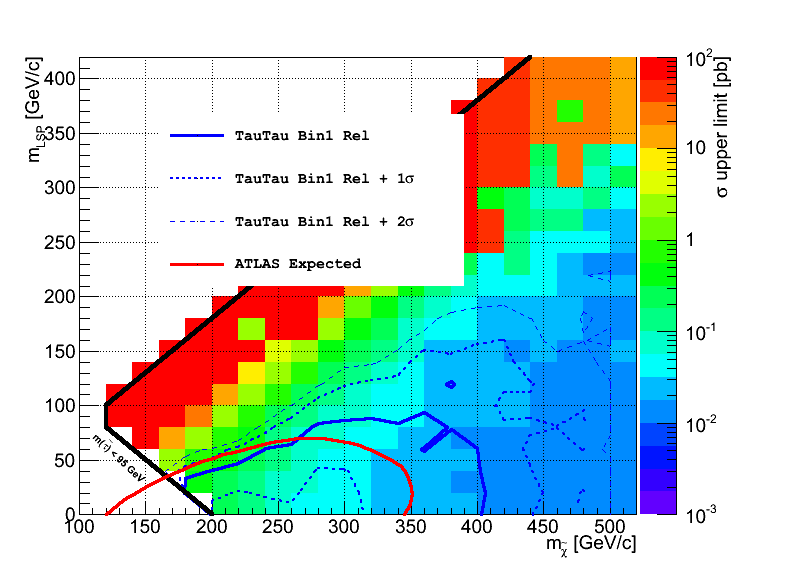
\includegraphics[width=0.49\textwidth,keepaspectratio=true]{StatisticsFig/NewFigs/TauTau_Bin1Rel.png}
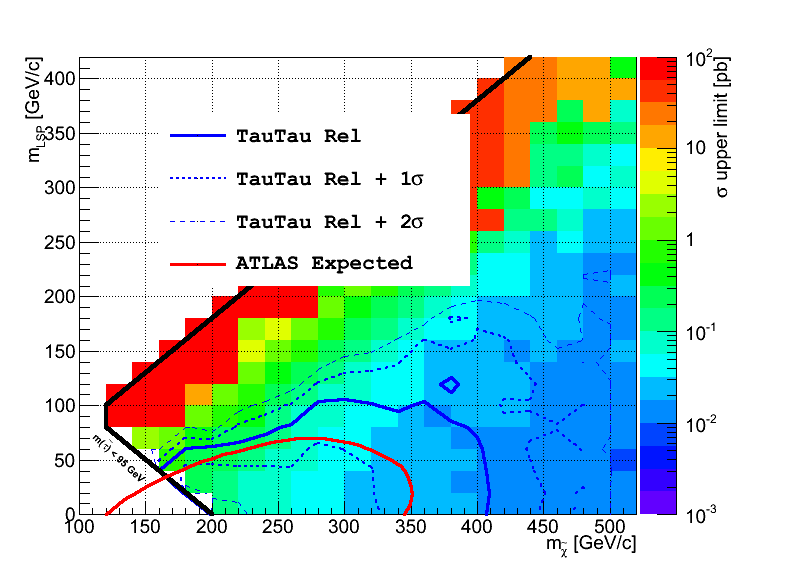
\includegraphics[width=0.49\textwidth,keepaspectratio=true]{StatisticsFig/NewFigs/TauTau_Bin1Rel_Bin2.png}
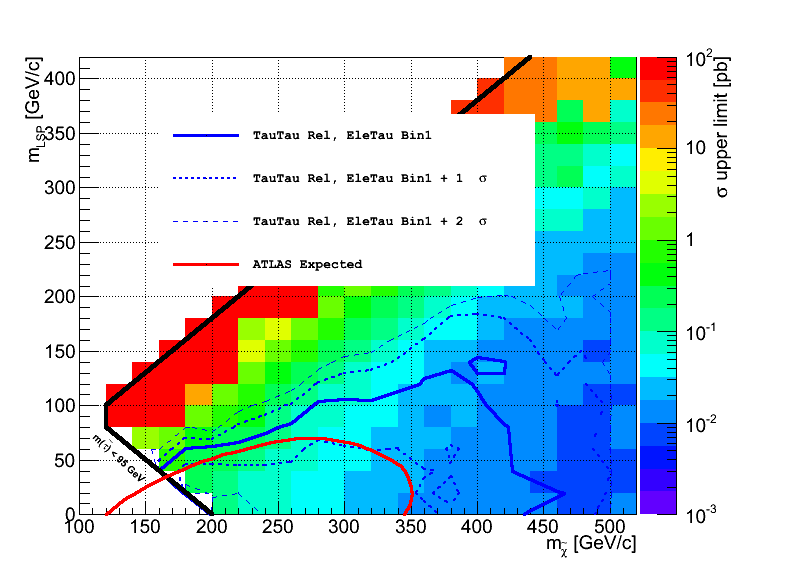
\includegraphics[width=0.49\textwidth,keepaspectratio=true]{StatisticsFig/NewFigs/TauTau_EleTauBin1.png}
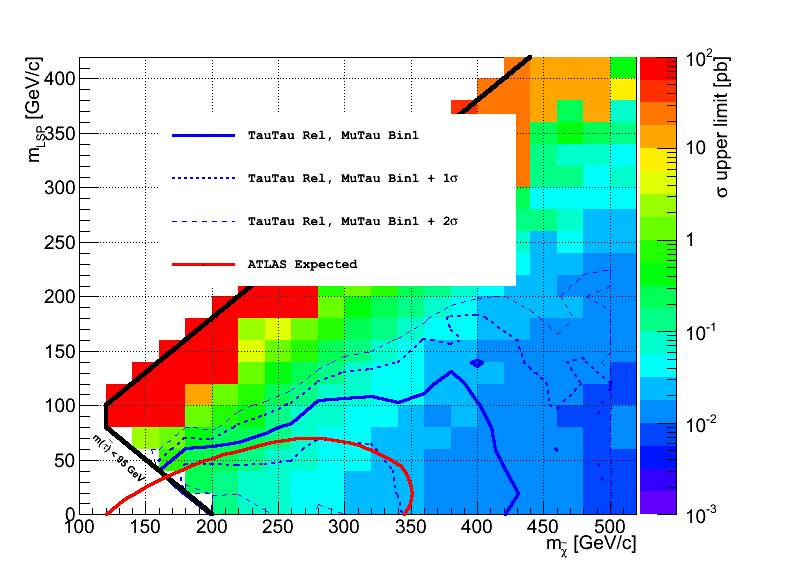
\includegraphics[width=0.49\textwidth,keepaspectratio=true]{StatisticsFig/NewFigs/TauTau_MuTauBin1.png}
\caption{}
\label{fig:limit_bins}
\end{figure}
\end{linenomath}
%%%%%%%%%%

%%%%%%%%%%
\begin{linenomath}
\begin{figure}[h]
\centering
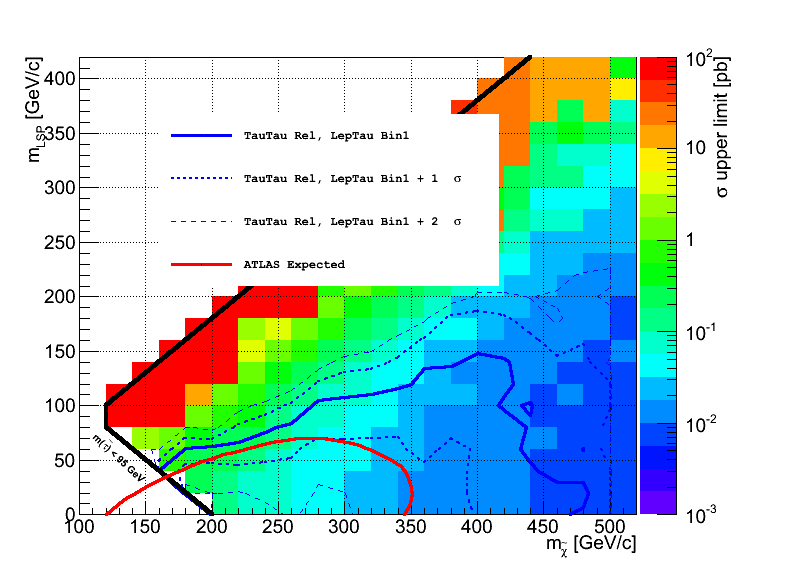
\includegraphics[width=0.9\textwidth,keepaspectratio=true]{StatisticsFig/NewFigs/Final_4BinRel.png}
\caption{}
\label{fig:limit_final}
\end{figure}
\end{linenomath}
%%%%%%%%%%
